%%%%%%%%%%%%%%%%%%%%%%%%%%%%%%%%%%%%%%%%%
% Beamer Presentation
% LaTeX Template
% Version 1.0 (10/11/12)
%
% This template has been downloaded from:
% http://www.LaTeXTemplates.com
%
% License:
% CC BY-NC-SA 3.0 (http://creativecommons.org/licenses/by-nc-sa/3.0/)
%
%%%%%%%%%%%%%%%%%%%%%%%%%%%%%%%%%%%%%%%%%

%----------------------------------------------------------------------------------------
%	PACKAGES AND THEMES
%----------------------------------------------------------------------------------------

\documentclass{beamer}

\mode<presentation> {

% The Beamer class comes with a number of default slide themes
% which change the colors and layouts of slides. Below this is a list
% of all the themes, uncomment each in turn to see what they look like.

%\usetheme{default}
%\usetheme{AnnArbor}
%\usetheme{Antibes}
%\usetheme{Bergen}
%\usetheme{Berkeley}
%\usetheme{Berlin}
%\usetheme{Boadilla}
%\usetheme{CambridgeUS}
%\usetheme{Copenhagen}
%\usetheme{Darmstadt}
%\usetheme{Dresden}
%\usetheme{Frankfurt}
%\usetheme{Goettingen}
%\usetheme{Hannover}
%\usetheme{Ilmenau}
%\usetheme{JuanLesPins}
%\usetheme{Luebeck}
\usetheme{Madrid}
%\usetheme{Malmoe}
%\usetheme{Marburg}
%\usetheme{Montpellier}
%\usetheme{PaloAlto}
%\usetheme{Pittsburgh}
%\usetheme{Rochester}
%\usetheme{Singapore}
%\usetheme{Szeged}
%\usetheme{Warsaw}

% As well as themes, the Beamer class has a number of color themes
% for any slide theme. Uncomment each of these in turn to see how it
% changes the colors of your current slide theme.

%\usecolortheme{albatross}
%\usecolortheme{beaver}
%\usecolortheme{beetle}
%\usecolortheme{crane}
%\usecolortheme{dolphin}
%\usecolortheme{dove}
%\usecolortheme{fly}
%\usecolortheme{lily}
%\usecolortheme{orchid}
%\usecolortheme{rose}
%\usecolortheme{seagull}
%\usecolortheme{seahorse}
%\usecolortheme{whale}
%\usecolortheme{wolverine}

%\setbeamertemplate{footline} % To remove the footer line in all slides uncomment this line
%\setbeamertemplate{footline}[page number] % To replace the footer line in all slides with a simple slide count uncomment this line

%\setbeamertemplate{navigation symbols}{} % To remove the navigation symbols from the bottom of all slides uncomment this line
}
\usepackage[utf8]{inputenc}
\usepackage{amsmath}
\usepackage[spanish,es-tabla]{babel}
\usepackage{graphicx} % Allows including images
\usepackage{booktabs} % Allows the use of \toprule, \midrule and \bottomrule in tables

%----------------------------------------------------------------------------------------
%	TITLE PAGE
%----------------------------------------------------------------------------------------

\title[Estructura fina]{Determinación experimental de la estructura fina} % The short title appears at the bottom of every slide, the full title is only on the title page

\author[Hernández A., Sánchez D.]{Alejandro Hernández A. \and Daniel Sánchez M.} % Your name
\institute[Uniandes] % Your institution as it will appear on the bottom of every slide, may be shorthand to save space
{
Universidad de los Andes, Bogotá, Colombia \\ % Your institution for the title page
%\medskip
%\textit{a.hernandez105@uniandes.edu.co}\\
%\textit{jd.prada1760@uniandes.edu.co}
 % Your email address
}
\date{Octubre 29, 2015} % Date, can be changed to a custom date

\begin{document}

\begin{frame}
\titlepage % Print the title page as the first slide
\end{frame}

\begin{frame}
\frametitle{Tabla de contenidos} % Table of contents slide, comment this block out to remove it
\tableofcontents % Throughout your presentation, if you choose to use \section{} and \subsection{} commands, these will automatically be printed on this slide as an overview of your presentation
\end{frame}

%----------------------------------------------------------------------------------------
%	PRESENTATION SLIDES
%----------------------------------------------------------------------------------------

%------------------------------------------------
\section{¿Qué es la estructura fina?} % Sections can be created in order to organize your presentation into discrete blocks, all sections and subsections are automatically printed in the table of contents as an overview of the talk
%------------------------------------------------

\section{Trabajos previos}


\section{Montaje experimental}

\subsection{Epectrómetro ESPARTACO}

\section{Resultados experimentales}

\subsection{Sodio}

\subsection{Hidrógeno}

\subsection{Deuterio}

\section{Perspectivas futuras}

\begin{frame}
\frametitle{¿Qué es la estructura fina?}
\ 


El espectro atómico predicho por el modelo de Bohr solo depende del número cuántico principal $n$, pero dicho modelos excluye \textbf{efectos relativistas} además del \textbf{spin electrónico}. La estructura fina describe el splitting de las líneas espectrales de diversos átomos debido a las correcciones introducidas por esos efectos en la ecuación de Schrödinger. \\\

El hamiltoniano total del sistema es

\begin{equation}
H = H_{0} + H_{kinetic} + H_{SO} + H_{Darwin}
\end{equation}
\end{frame}

%------------------------------------------------

\begin{frame}
\frametitle{¿Qué es la estructura fina?}
\begin{itemize}
	\item \textbf{Término cinético} $H_{kinetic} = - \frac{p^4}{8m^3c^2}$
	\\\
	
	
	$K = \sqrt{p^2c^2 + m^2c^4} - mc^2 = \frac{p^2}{2m} - \frac{p^4}{8m^3c^2} + \cdots$
	\
	\\
	\
	\\
	
	\item \textbf{Término Spín-Órbita} $H_{SO} = \frac{1}{2} \left( \frac{Ze^2}{4 \pi \epsilon_{0}} \right) \left( \frac{g_{s}}{2m^2c^2} \right) \frac{\vec{L}\cdot \vec{S}}{r^3}$
	\
	\\
	\
	\\
	
	\item \textbf{Término Darwiniano} $H_{Darwin} = \frac{\hbar^2}{8m^2c^2}\ 4 \pi \left( \frac{Ze^2}{4 \pi \epsilon_{0}} \right)$
	\
	\\
	\
	\\
\end{itemize}
\
\\
\textbf{Efecto total} $\Delta E = \frac{E_{n}(Z\alpha)^2}{n}\left( \frac{1}{j+\frac{1}{2}} - \frac{3}{4n} \right)$
\
\\
\
\\


El \textbf{objetivo de este proyecto} es evidenciar los efectos previamente mencionados al comprobar que la separación entre las líneas espectrales es proporcional a $(Z\alpha)^2$, donde $\alpha = \frac{1}{4 \pi \epsilon_{0}}\frac{e^2}{\hbar c}$ es la constante de estructura fina y $Z$ es el número atómico.
\end{frame}

%------------------------------------------------

\begin{frame}[fragile] % Need to use the fragile option when verbatim is used in the slide
\frametitle{Trabajos Previos}

\begin{itemize}
	\item Acosta J., Ramírez D., Proyecto final de laboratorio Intermedio, 2015-1.
	\
	\\ 
	\
	\\
	
	\item Laboratorio de Física Moderna.
	\
	\\
	\
	\\
	
	\item Diversos proyectos del profesor Benjamín Oostra.
	
\end{itemize}
\end{frame}

%------------------------------------------------

%\begin{frame}
%\frametitle{Multiple Columns}
%\begin{columns}[c] % The "c" option specifies centered vertical alignment while the "t" option is used for top vertical alignment
%
%\column{.45\textwidth} % Left column and width
%\textbf{Heading}
%\begin{enumerate}
%\item Statement
%\item Explanation
%\item Example
%\end{enumerate}
%
%\column{.5\textwidth} % Right column and width
%Lorem ipsum dolor sit amet, consectetur adipiscing elit. Integer lectus nisl, ultricies in feugiat rutrum, porttitor sit amet augue. Aliquam ut tortor mauris. Sed volutpat ante purus, quis accumsan dolor.
%
%\end{columns}
%\end{frame}

%------------------------------------------------

%------------------------------------------------

%\begin{frame}
%\frametitle{Table}
%\begin{table}
%\begin{tabular}{l l l}
%\toprule
%\textbf{Treatments} & \textbf{Response 1} & \textbf{Response 2}\\
%\midrule
%Treatment 1 & 0.0003262 & 0.562 \\
%Treatment 2 & 0.0015681 & 0.910 \\
%Treatment 3 & 0.0009271 & 0.296 \\
%\bottomrule
%\end{tabular}
%\caption{Table caption}
%\end{table}
%\end{frame}

%------------------------------------------------

\begin{frame}
\frametitle{Montaje experimental}
\begin{itemize}
	\item\textbf{Espectrómetro ESPARTACO} 
	\begin{figure}[h!]
		\centering
		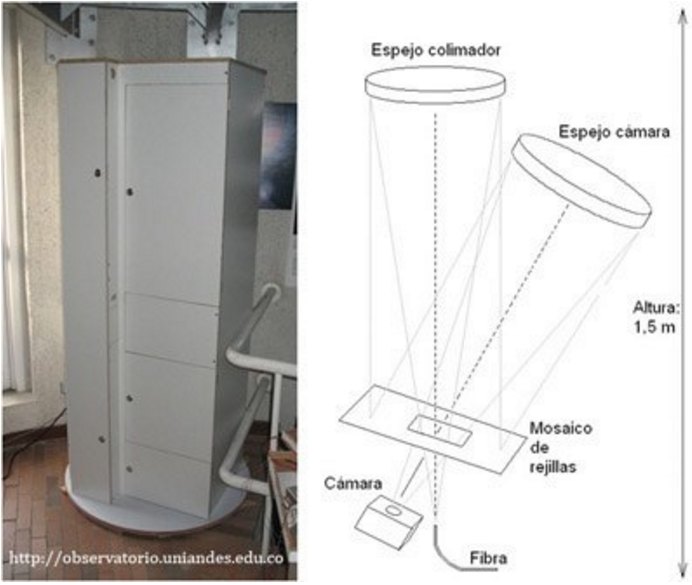
\includegraphics[width=0.5\textwidth]{espectrometro}
		\caption{Dispositivo ESPARTACO en el observatorio del edificio H.}
	\end{figure}
\end{itemize}

\end{frame}

%------------------------------------------------



%------------------------------------------------

\begin{frame}
\frametitle{Otros elementos utilizados}
\begin{itemize}
	\item \textbf{Tubos contenedores de gases}
		\begin{figure}[h!]
			\centering
			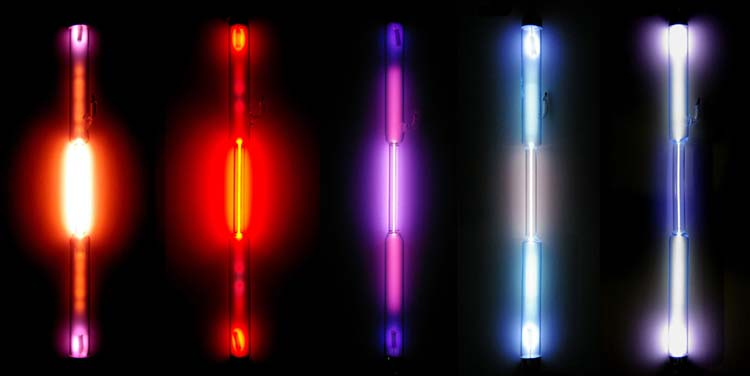
\includegraphics[width=0.2\textwidth,height = 0.2\textheight]{tubes}
			\caption{Diversos gases confinados en tubos especiales.}
		\end{figure}
	\item \textbf{Base}
		\begin{figure}[h!]
			\centering
			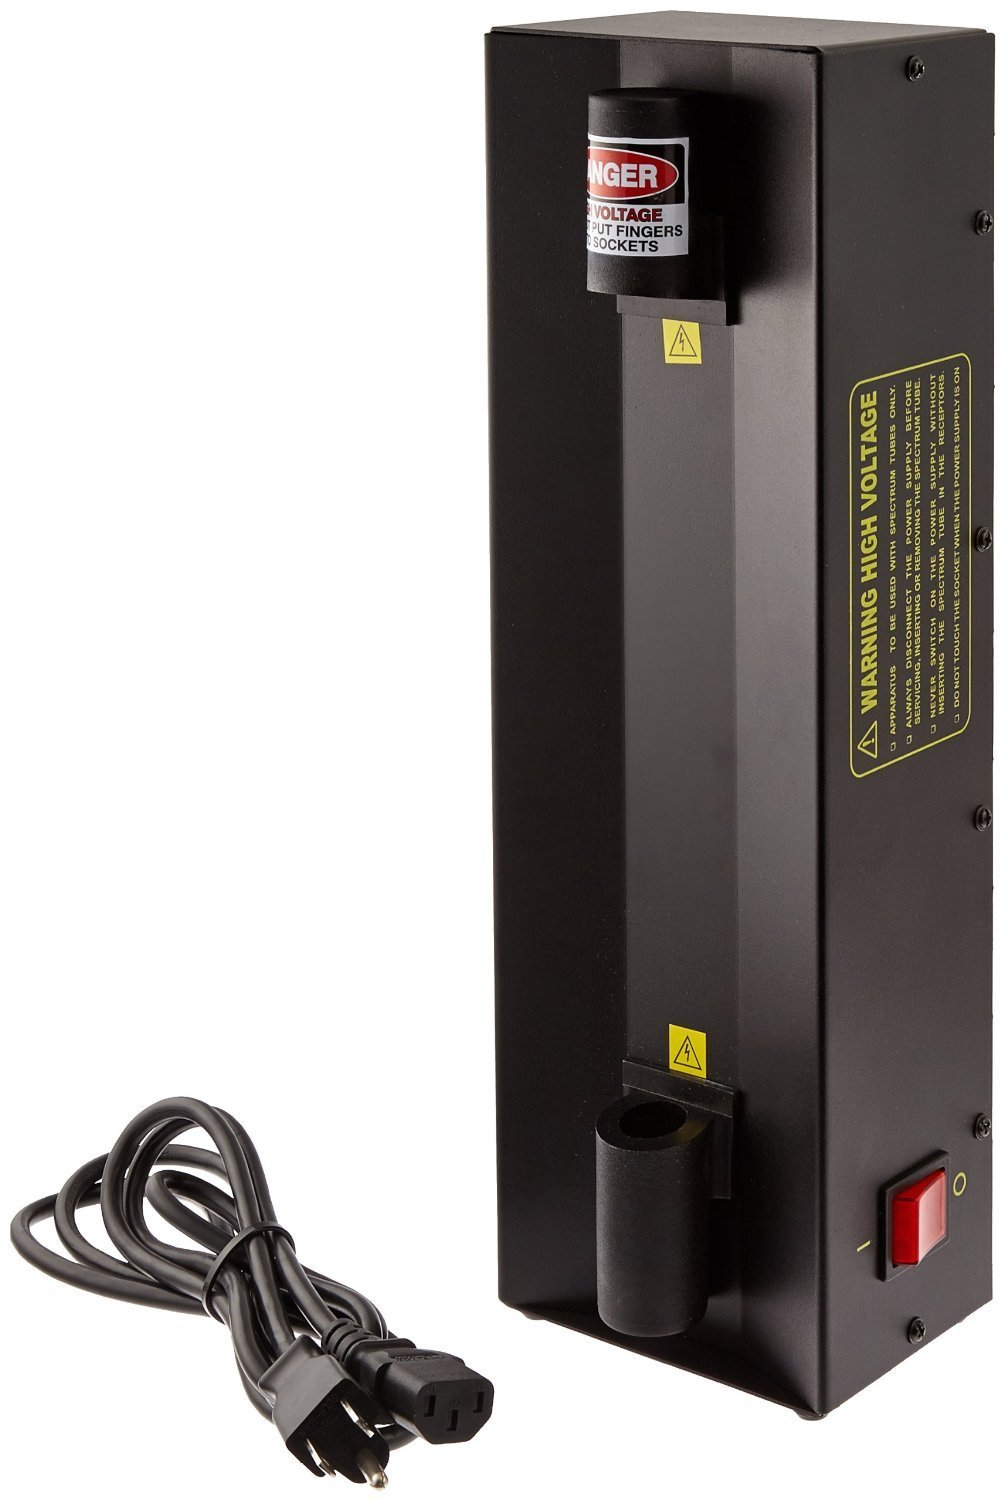
\includegraphics[width=0.2\textwidth,height = 0.3\textheight]{base}
			\caption{Base para poner los tubos.}
		\end{figure}
\end{itemize}
\end{frame}

%------------------------------------------------

\begin{frame}[fragile] % Need to use the fragile option when verbatim is used in the slide
\frametitle{Metodología}
%An example of the \verb|\cite| command to cite within the presentation:\\~
%
%This statement requires citation \cite{p1}.
\begin{itemize}
	\item Exponer el gas de calibración y el gas al cual se desea medir estructura fina al "lente" de ESPARTACO.
	\
	\\
	
	\
	\\
	
	\item Recopilación de datos con un software basado en MIDAS \cite{midas}.
	\
	\\
	
	\
	\\
	
	\item Verificar una "buena" toma de datos.
	\
	\\
	
	\
	\\
	
	\item Análisis de datos con el software IRIS \cite{iris}
\end{itemize}

\end{frame}

\begin{frame}[fragile]
\frametitle{Resultados experimentales - Sodio}
\begin{figure}[h!]
	\centering
	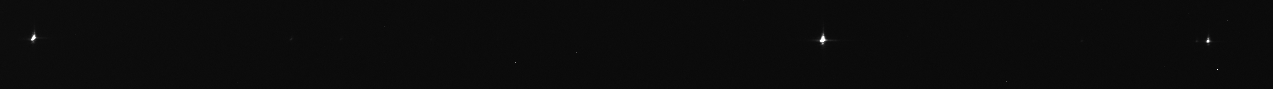
\includegraphics[width=1.\textwidth,height = 0.1\textheight]{neon-sodio}
	\caption{Neón-Sodio.}
\end{figure}

\begin{figure}[h!]
	\centering
	
\includegraphics[width=1.\textwidth,height = 0.1\textheight]{co-sodio}
	\caption{Sodio.}
\end{figure}

\begin{figure}[h!]
	\centering
	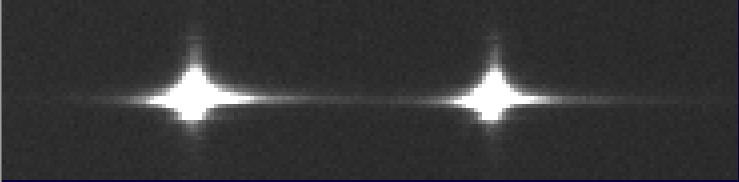
\includegraphics[width=1.\textwidth,height = 0.15\textheight]{sodio}
	\caption{Sodio.}
\end{figure}


\end{frame}

\begin{frame}[fragile]
	\frametitle{Resultados experimentales - Sodio}
	\begin{figure}[h!]
		\centering
		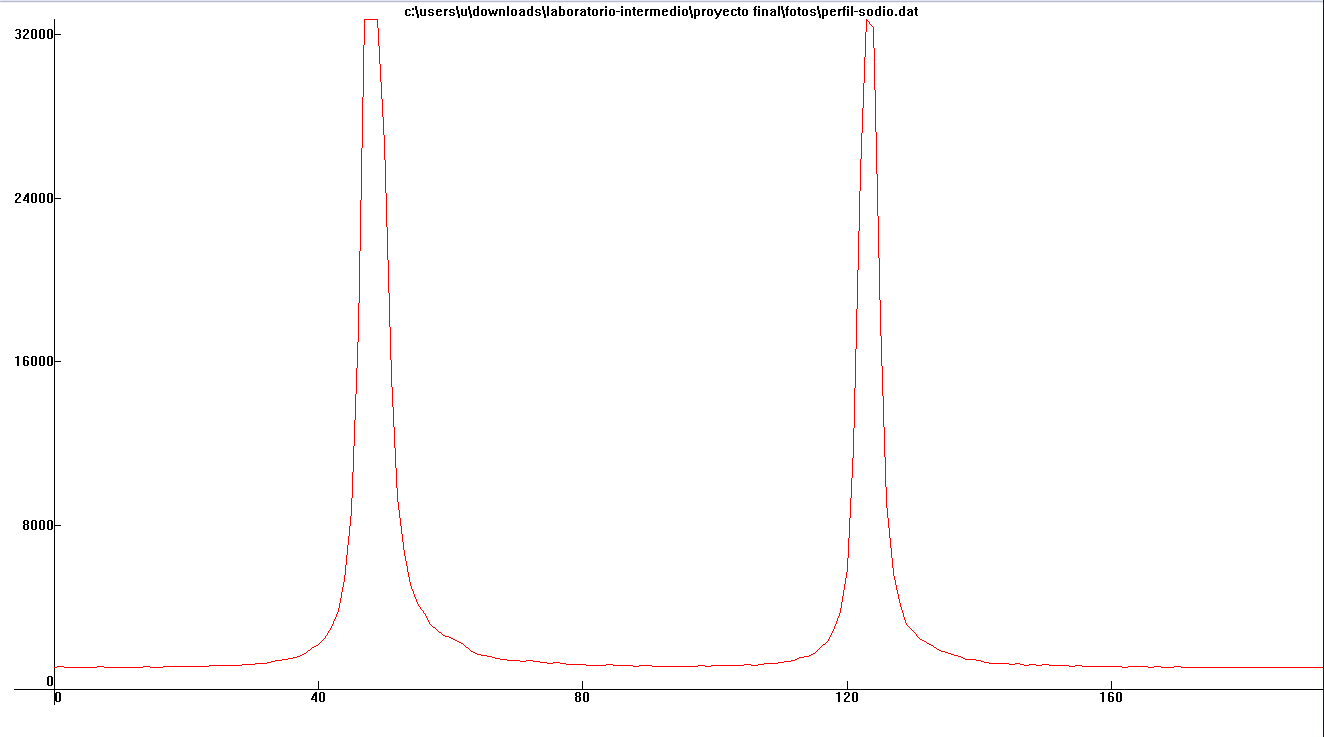
\includegraphics[width=1.\textwidth,height = 0.7\textheight]{perfil-sodio}
		\caption{Perfil-Sodio.}
	\end{figure}
	

\end{frame}

\begin{frame}[fragile]
	\frametitle{Resultados experimentales - Sodio}

Fit lineal de los datos: $y = 7.65\cdot 10^-3 x + 586.77$,   $r^2 = 0.999971225$  
\
\\

\
\\

Separación en pixeles: $76$
\
\\

\
\\

Separación en longitud de onda: $0.58\ nm$
\
\\

\
\\

Separación teórica: $ 0.59\ nm$
\
\\

\
\\

Error porcentual: $ 2.66\% $

	
	
\end{frame}

\begin{frame}[fragile]
	\frametitle{Resultados experimentales - Hidrógeno - Deuterio}
	\begin{figure}[h!]
		\centering
		
\includegraphics[width=1.\textwidth,height = 0.1\textheight]{neon-hid}
		\caption{Neón-Hidrógeno.}
	\end{figure}
	
	\begin{figure}[h!]
		\centering
		
\includegraphics[width=1.\textwidth,height = 0.1\textheight]{co-hid}
		\caption{Hidrógeno.}
	\end{figure}
	
	\begin{figure}[h!]
		\centering
		
\includegraphics[width=1.\textwidth,height = 0.1\textheight]{co-deu}
		\caption{Deuterio.}
	\end{figure}
\end{frame}


\begin{frame}[fragile]
	\frametitle{Resultados experimentales - Hidrógeno - Deuterio}
	\begin{figure}[h!]
		\centering
		
\includegraphics[width=1.\textwidth,height = 0.1\textheight]{neon-hid}
		\caption{Neón-Hidrógeno.}
	\end{figure}
	
	\begin{figure}[h!]
		\centering
		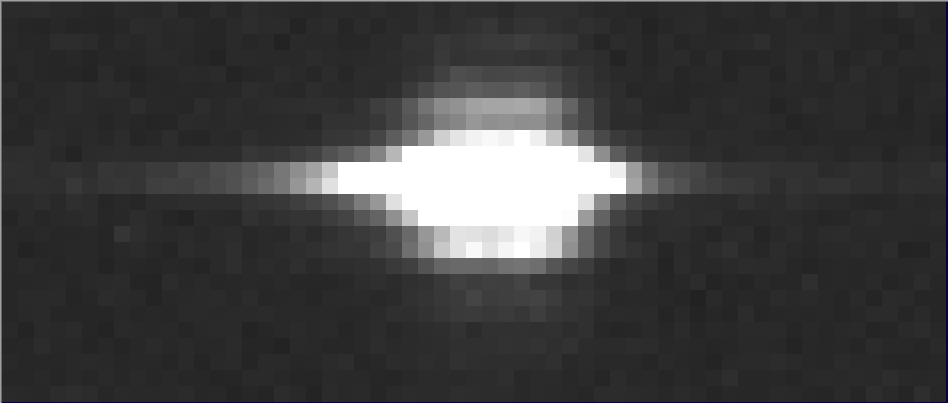
\includegraphics[width=.7\textwidth,height = 0.1\textheight]{hid}
		\caption{Hidrógeno.}
	\end{figure}
	
	\begin{figure}[h!]
		\centering
		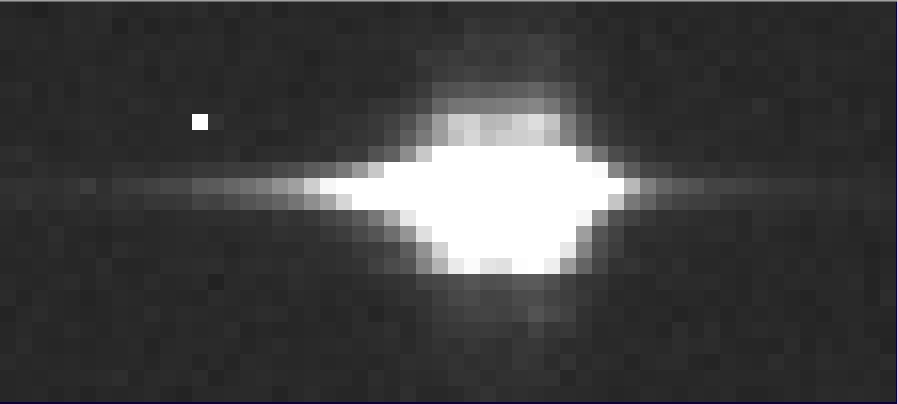
\includegraphics[width=.7\textwidth,height = 0.1\textheight]{deu}
		\caption{Deuterio.}
	\end{figure}
\end{frame}

\begin{frame}[fragile]
	\frametitle{Resultados experimentales - Hidrógeno - Deuterio}
	\begin{figure}[h!]
		\centering
		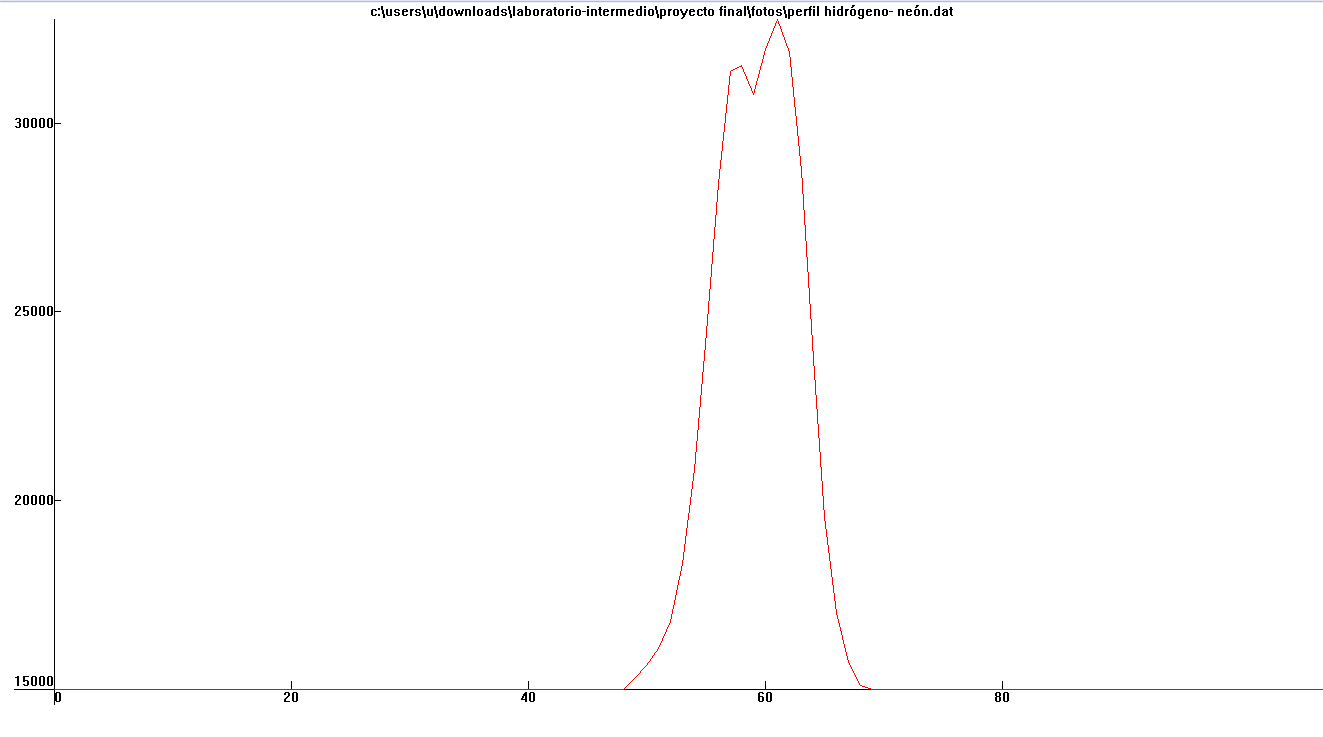
\includegraphics[width=1.\textwidth,height = 0.7\textheight]{perfil-hid}
		\caption{Perfil-Hidrógeno.}
	\end{figure}
	
\end{frame}

\begin{frame}[fragile]
	\frametitle{Resultados experimentales - Hidrógeno - Deuterio}
	\begin{figure}[h!]
		\centering
		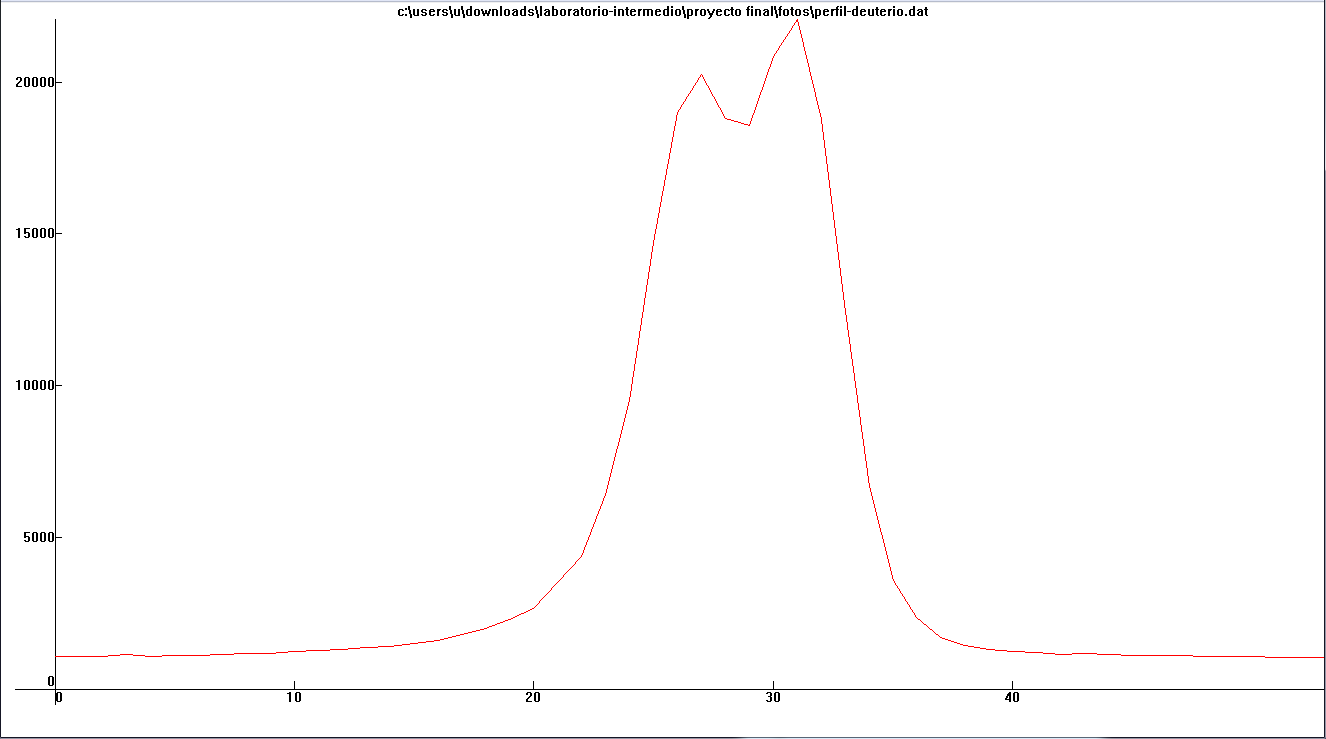
\includegraphics[width=1.\textwidth,height = 0.7\textheight]{perfil-deu}
		\caption{Perfil-Deuterio.}
	\end{figure}
	
\end{frame}

\begin{frame}[fragile]
	\frametitle{Resultados experimentales - Hidrógeno - Deuterio}
	
	Fit lineal de los datos: $y = 7.65\cdot 10^-3 x + 586.77$,   $r^2 = 0.999971225$  
	\
	\\
	
	\
	\\
	
	Separación en pixeles Hidrógeno: $3$
	\
	\\
	
	\
	\\
	
	Separación en pixeles Deuterio: $4$
	\
	\\
		
	\
	\\
		
	Separación en longitud de onda Hidrógeno: $0.008\ nm$
	\
	\\
	
	\
	\\
	
	Separación en longitud de onda Deuterio: $0.012\ nm$
	\
	\\
	
	\
	\\
	
	Separación teórica: $ 0.016\ nm$
	\
	\\
	
	\
	\\
	
	Error porcentual Hidrógeno: $ 43.9\% $
	\
	\\
	
	\
	\\
	
	Error porcentual Deuterio: $ 25.2\% $
	
	
	
\end{frame}

\begin{frame}[fragile]
	\frametitle{Perspectivas futuras}
	
	\begin{itemize}
		\item Verificar la proporcionalidad a $(Z\alpha^2)$.
		\
		\\
		
		\
		\\
		
		\item Realizar mediciones para otros gases, entre ellos, helio, cadmio, mercurio y zinc.
		\
		\\
		
		\
		\\
		
		\item Realizar nuevamente las mediciones para hidrógeno y deuterio con el fin de reducir los errores porcentuales obtenidos.		
		
	\end{itemize}	
	
\end{frame}

%------------------------------------------------

\begin{frame}
\frametitle{References}
\footnotesize{
\begin{thebibliography}{99} % Beamer does not support BibTeX so references must be inserted manually as below
\bibitem[2]{iris} IRIS. 
\newblock Software para análisis espectográfico obtenido de \emph{http://www.astrosurf.com/buil/us/iris/iris.htm}


\bibitem[1]{midas} MIDAS
\newblock Software para el procesamiento de imágenes desarrollado por ESO, cuya información se encuentra en
\emph{http://www.eso.org/sci/data-processing/software/esomidas/}

\bibitem[3]{cohen} Cohen-Tannoudji et al. (1992)
\newblock Quantum Mechanics Volume II
\newblock Cap. XII, págs. 1247 -- 1257.

\bibitem[4]{oostra} Oostra B., Ramírez D. (2011)
\newblock Espartaco: A High-Resolution, Low-Cost Spectrograph For Students 
\newblock \emph{Revista Colombiana de Física} 43(2), 312 -- 317.
\end{thebibliography}
}
\end{frame}

%------------------------------------------------

\begin{frame}
\Huge{\centerline{Gracias...totales.}}
\end{frame}

%----------------------------------------------------------------------------------------

\end{document} 